\documentclass[tikz,border=6pt]{standalone}

\usepackage{amsmath,amssymb}
\usetikzlibrary{calc,arrows.meta,shapes.geometric}

\begin{document}

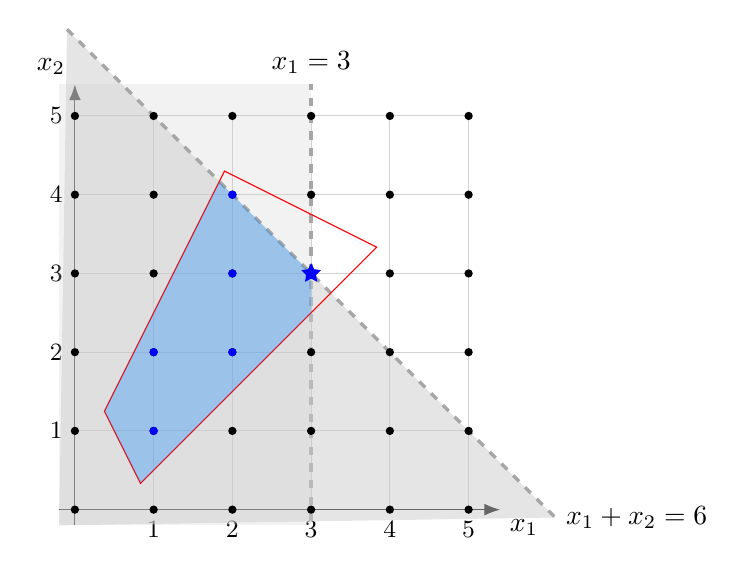
\begin{tikzpicture}[scale=1.0]
  % axes
  \draw[-{Latex[length=2mm]}] (-0.2,0) -- (5.4,0) node[below right] {$x_1$};
  \draw[-{Latex[length=2mm]}] (0,-0.2) -- (0,5.4) node[above left] {$x_2$};

  % light grid guides + tick labels (drawn first)
  \foreach \i in {1,...,5} {
    \draw[gray!35] (\i,0) -- (\i,5);
    \draw[gray!35] (0,\i) -- (5,\i);
    \node[below] at (\i,-0.03) {\small \i};
    \node[left]  at (-0.03,\i) {\small \i};
  }

  % === Halfspace cut 1: x_1 <= 3 (shade in gray and draw the cut line) ===
  \def\cutx{3}
  \path[fill=gray!40,opacity=0.25]
    (-0.2,-0.2) -- (\cutx,-0.2) -- (\cutx,5.4) -- (-0.2,5.4) -- cycle;
  \draw[gray!70,very thick,dashed] (\cutx,-0.15) -- (\cutx,5.4)
    node[above,black] {$x_1=3$};

  % === Halfspace cut 2: x_1 + x_2 <= 6 (draw the cut line) ===
   \path[fill=gray!40,opacity=0.5]
    (-0.2,-0.2) -- (-0.1,6.1) -- (6.1,-0.1)-- cycle;
  \draw[gray!70,very thick,dashed] (-0.1,6.1) -- (6.1,-0.1)
    node[anchor=west,black] {$x_1+x_2=6$};

  % original feasible polygon vertices
  \def\vAD{(0.375,1.25)}           % A ∩ D
  \def\vCD{(0.833333,0.333333)}    % C ∩ D
  \def\vBC{(3.833333,3.333333)}    % B ∩ C
  \def\vAB{(1.9,4.3)}              % A ∩ B

  % intersections with the cuts
  \coordinate (Xlow) at (3,2.5);                     % x1=3 with x1-x2=0.5
  \coordinate (Xtop) at (3,3.0);                     % x1=3 with x1+x2=6
  \coordinate (XE)   at (11/6,25/6);                 % (-2x1+x2=0.5) with (x1+x2=6)

  % --- Original feasible region outline (kept in red)
  \draw[red] \vAD -- \vCD -- \vBC -- \vAB -- cycle;

  % --- New feasible region after both cuts: fill with a different blue tone
  % Order: vCD -> Xlow -> Xtop -> XE -> vAD -> back to vCD
  \fill[blue!50!cyan,opacity=0.3]
    \vCD -- (Xlow) -- (Xtop) -- (XE) -- \vAD -- cycle;

  % --- Lattice points: draw AFTER fills so they appear on top
  \foreach \i in {0,...,5} {
    \foreach \j in {0,...,5} {
      \fill[black] (\i,\j) circle (1.5pt);
    }
  }

  % Feasible integer grid points (under both cuts), drawn on top
  \foreach \P in {(1,1),(1,2),(2,2),(2,3),(3,3),(2,4)}{
    \fill[blue] \P circle (1.5pt);
  }

  % === New LP optimum with both cuts: lies at (3,3) on x1+x2=6 and x1=3 ===
  \coordinate (optboth) at (3,3);
  \node[star,star points=5,star point ratio=2.0,fill=blue,draw=blue,scale=0.35] at (optboth) {};
\end{tikzpicture}

\end{document}
